\documentclass[12pt]{article}
\usepackage[margin=0.75in]{geometry}
\usepackage{graphicx}
\usepackage{multicol}
\usepackage{float}
\usepackage{upgreek}

% for dots in TOC:
\usepackage{tocloft}
\renewcommand{\cftsecleader}{\cftdotfill{\cftdotsep}}

\setlength{\parindent}{0mm}

\begin{document}

{\centering
\LARGE Physics I-II Lab Manual \par
}
\hfill \break

{\centering
\large Preface \par
}
\hfill \break \vspace{-4mm}

This is the lab manual for Physics 2211L, 2212L, 1111L, and 1112L taught by Dr. Nathan Harrison.
In some labs you will have to copy and paste small amounts of code;
it is recommended that you copy from the the original \LaTeX \ source, \textit{not} from the PDF file which often leads to formatting errors.
Another common mistake is to not unzip the Java-based simulations;
if the simulation opens but the screen is blank it is because you didn't unzip the file.
\vfill
\textcopyright \ Nathan Harrison 2018
\pagebreak \clearpage

\tableofcontents
\pagebreak \clearpage

\input{surfaceAreaVolumeDensity.tex}
\input{fitting1Dmotion.tex}
\input{projectileMotion.tex}
\input{forces.tex}
\input{energy.tex}
\section{Work and Power}

\underline{\textbf{Part 1}} \par
Use a constant horizontal force to push a block ($v_i = 0$) up a ramp that has friction.
Choose and record all relevant values.
Identify all forces present, label each one as conservative or non-conservative, and calculate the amount of work each one does on the block.
Use these work values to calculate the expected final velocity after some time interval.
Compare this calculation to the final velocity measured by IP.

\begin{figure}[H]
\includegraphics[scale=0.50]{figures/workPower/fig1.png}
\end{figure}


\underline{\textbf{Part 2}} \par
In this lab you will conduct a real life experiment to calculate your (or a lab mate's) maximum power output, with an uncertainty.

\begin{enumerate}
\item Write down your weight (with uncertainty) and convert to mass (in kg).
\item Gather relevant supplies (a ruler, stopwatch/smartphone, paper, pencil, and calculator) and go as a class to the staircase next to the Nesbitt building.
\item Use your ruler to measure the height of one stair. Also count the number of stairs to get the total elevation change from the bottom to the top. Make sure to propagate the error.
\item Have one person control the stop watch while another person runs up the hill next to the staircase as fast as possible. Record the time taken, with uncertainty. The runner and timer should coordinate a strategy so that the runner's velocity at the bottom is approximately equal to the velocity at the top; that way the change in energy is only due to the change in height. Include your strategy in your lab report. Although your stopwatch probably has very good precision, you may want to assign a larger time uncertainty due to the human error of starting and stopping at the right time.
\item Write down the relevant equations from class and calculate your power with uncertainty. Give your answer both in W and hp.
\end{enumerate}

In the event of bad weather, you may do the following experiment instead.
Here you will measure your maximum power by jumping as high as you can.
In this part you will measure your maximum power by jumping as high as you can.
\begin{enumerate}
\item Use a meter stick to measure the three relevant heights shown in the figure (with uncertainty).
\item Also write down your weight (converted to kg, with uncertainty).
\item Assume constant acceleration and force, and use kinematics to calculate relevant velocities and time intervals. Also calulate the uncertainty in these quantities using error propagation.
\item Finally, calculate your power during the jump with uncertainty. Record your result in Watts and horsepower.
\end{enumerate}

\begin{figure}[H]
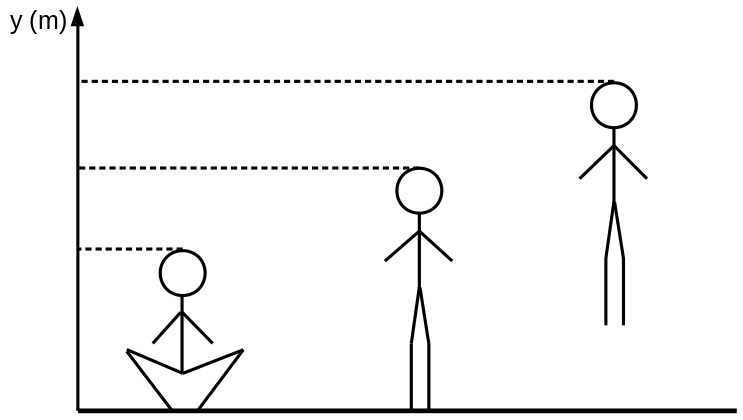
\includegraphics[scale=0.50]{figures/workPower/fig2.png}
\end{figure}

\pagebreak \clearpage

\input{momentum.tex}
\section{Torque}

\underline{\textbf{Part 1}} \par

\begin{verbatim}
https://phet.colorado.edu/sims/html/balancing-act/latest/balancing-act_en.html
Click "Game"
Complete all 4 levels - take screenshots of your results
\end{verbatim}

\underline{\textbf{Part 2}} \par

Background: it is well known that the harmonic series

\begin{equation}
\sum_{n=1}^{\infty} \frac{1}{n} = \frac{1}{1} + \frac{1}{2} + \frac{1}{3} + \frac{1}{4} + \dots
\end{equation}

aproaches infinity (albeit very slowly).
The similar sum

\begin{equation}
\sum_{n=1}^{\infty} \frac{1}{n^2} = \frac{1}{1^2} + \frac{1}{2^2} + \frac{1}{3^2} + \frac{1}{4^2} + \dots
\end{equation}

was first posed in 1650 and not solved until 1734 by Leonhard Euler.
Euler showed that this sum converges to $\pi^2$/6.

\vspace{\baselineskip}

Confirm Euler's result with the following experiment in Interactive Physics.
\begin{enumerate}
\item Create a beam of length 2 $m$ balanced at the center.
\item Put a 1 $kg$ mass 1 $m$ from the center, a 1/2 $kg$ mass 1/2 $m$ from the center, a 1/3 $kg$ mass 1/3 $m$ from the center, etc.
\item On the opposite edge of the beam, place a single mass. Decide what this mass should be to balance the system and explain how this confirms Euler's result.
\end{enumerate}

\begin{figure}[H]
\includegraphics[scale=0.50]{figures/torque/fig1.png}
\end{figure}

\pagebreak \clearpage

\input{angularKinematics.tex}
\input{orbits.tex}
\input{waves.tex}
\input{dopplerEffect.tex}
\section{Chaos}

In this lab you will study some interesting properties of chaotic systems.

\vspace{\baselineskip}

\underline{\textbf{Part 1}} \par
Draw 3 points on a piece of paper to form a triangle.
Label the points 0, 1, and 2.
Also randomly draw a 4th point - this will be the starting point of the experiment.
Next, randomly generate either a 0, 1, or 2 (e.g. by rolling dice), the number generated will correspond to one of the corners of the triangle.
Make a new point halfway between the starting point and the corner of the triangle selected in the previous step; this point becomes the new starting point for the next iteration.
Repeat this process of making new points halfway between the last point and the corner of the triangle randomly selected many times.

\vspace{\baselineskip}

Do at least 10 points by hand until you get the idea.
Your final result should contain at least 2000 points.
If you are a student who insists that learning basic coding is not useful then you can do all 2000 points by hand.
Otherwise, try the following SageMath script.

\begin{verbatim}
# Create a graphics object to display the points
g = Graphics()


# Add 3 points that make up a triangle
tri = [ (1, 1), (3, 1), (2, 3) ]
g += point(tri, color="red", size=35)


# Choose a random starting point
x = 2.6 
y = 1.3 
g += point((x, y), color="black", size=10)


# Generate random numbers (0, 1, or 2)
# corresponding to points on the triangle.
# For each iteration, move halfway from the 
# last point to the chosen triangle point.

nPts = 2500
for i in range(0, nPts):
  rand = ZZ.random_element(0, 3)
  x = x + 0.50*(tri[rand][0] - x) # experiment with the fraction
  y = y + 0.50*(tri[rand][1] - y) # experiment with the fraction
  g += point((x, y), color="black", size=10)


g.show()
\end{verbatim}

% some interesting results:
% 0.25 total randomness
% 0.5 perfect fractal pattern
% 0.8 3 groups of 3 groups of 3 groups

% TODO Add barnsley fern example

\pagebreak \clearpage


\end{document}
